% !TEX root = main.tex
% ============================================================================
% CHAPTER 3: PROPOSED ALGORITHM
% ============================================================================

\chapter{معرفی الگوریتم پیشنهادی}
\section{مقدمه}

این فصل به تشریح دقیق الگوریتم پیشنهادی رمزنگاری تصاویر رنگی اختصاص دارد. هدف اصلی، ارائه توضیح شفاف، جامع و دقیق از هر یک از مراحل فرآیند رمزنگاری و رمزگشایی است به‌گونه‌ای که قابل بازتولید و ارزیابی مستقل باشد. نوآوری اصلی این پژوهش در به‌کارگیری ترکیبی پویا و چندلایه از ۹ سیستم آشوبی نمایی در کنار سیستم پیوسته سه‌بعدی \lr{Chen} برای جایگشت نهفته است؛ رویکردی که موجب ارتقاء چشمگیر امنیت در برابر انواع حملات تحلیل آماری، حملات تفاضلی و جستجوی فراگیر می‌شود.

ساختار این فصل بر چهار محور اصلی استوار است: نخست، مرور مؤلفه‌های آشوبی منتخب و نقش هر یک در ساختار رمز؛ دوم، تشریح گام‌به‌گام فرآیند رمزنگاری و فرآیند معکوس رمزگشایی همراه با روابط ریاضی و تعریف دقیق نمادها؛ سوم، اثبات ریاضی و تحلیل فضای کلید؛ و چهارم، معرفی روش پیاده‌سازی، مجموعه‌های داده مرجع و معیارهای ارزیابی استاندارد.

\section{نقش و پیکربندی سیستم‌های آشوبی منتخب}

همان‌گونه که مبانی نظری و روابط سیستم‌های آشوبی در فصل دوم به‌تفصیل تشریح گردید، در الگوریتم پیشنهادی از دو دسته سیستم آشوبی با اهداف متمایز استفاده شده است:

\begin{enumerate}
    \item \textbf{سیستم پیوسته سه‌بعدی \lr{Chen} برای مرحله جایگشت:} به دلیل فضای فاز سه‌بعدی پیچیده و نمای لیاپانوف مثبت بزرگ ($\lambda_1 \approx 2.03$)، مولفه $x(t)$ حاصل از حل عددی این سیستم با شرایط اولیه $(x_0, y_0, z_0)$ و پارامترهای استاندارد $a=35, b=3, c=28$ با استفاده از روش رانگ-کوتای مرتبه ۴ و ۵ (\lr{RK45}) با گام زمانی $dt=0.002$ حل می‌شود تا بردار جایگشت موقعیت مکانی پیکسل‌ها را تولید کند\cite{ref6}.
    \item \textbf{نگاشت‌های آشوبی نمایی (\lr{ECM}) برای مرحله انتشار:} ترکیب ۹ سیستم آشوبی نمایی مندرج در جدول ۲-۲ به دلیل داشتن دامنه آشوب پایدار گسترده و توزیع مقادیر در بازه $[0, 1)$ به کار گرفته شده‌اند. برای هر پیکسل، نوع نگاشت به‌صورت مستقل و پویا توسط یک نگاشت انتخاب‌گر لجستیک تعیین می‌گردد\cite{ref4}.
\end{enumerate}

\section{الگوریتم پیشنهادی: تشریح گام‌به‌گام}

الگوریتم رمزنگاری پیشنهادی از پنج مرحله متوالی تشکیل شده است. در ادامه، هر مرحله با جزئیات کامل ریاضی و توضیحات مفهومی تشریح می‌شود.

\subsection{مرحله ۱: تولید کلیدهای اولیه و آماده‌سازی}

در این مرحله، تمام پارامترهای اولیه الگوریتم مقداردهی می‌شوند. کلید رمزنگاری $K$ شامل هفت عدد مثبت پیوسته با دقت ۱۵ رقم اعشار مطابق رابطه زیر است:
\begin{equation}
K = \{x_0, y_0, z_0, x_{\mathrm{sel},0}, x_{\mathrm{ecm},0}, \mu, x_{\mathrm{final},0}\}
\label{eq:ch3-key-tuple}
\end{equation}

تصویر رنگی ورودی با ابعاد $H \times W \times 3$ بارگذاری شده و به سه کانال رنگی قرمز (\lr{R})، سبز (\lr{G}) و آبی (\lr{B}) تفکیک می‌شود. هر کانال به ابعاد $H \times W$ به‌صورت مستقل پردازش می‌گردد. تعداد کل پیکسل‌های هر کانال برابر با $N = H \times W$ است.

به‌منظور حذف حالت گذرای اولیه سیستم آشوبی\footnote{\lr{Transient State}} و اطمینان از قرارگیری سیستم در ناحیه آشوبی پایدار، سیستم \lr{Chen} برای ۱۰۰۰ گام زمانی اولیه اجرا شده و مقادیر حاصل دور انداخته می‌شوند (دوره \lr{warm-up}). این عمل یک الزام علمی در رمزنگاری آشوبی برای قطع هرگونه وابستگی مستقیم بین مقادیر اولیه کلید و خروجی اولیه است.

\subsection{مرحله ۲: جایگشت پیکسل‌ها با سیستم \lr{Chen}}

هدف این مرحله، از بین بردن همبستگی مکانی بالا بین پیکسل‌های مجاور در تصویر اصلی از طریق جابه‌جایی شبه‌تصادفی موقعیت مکانی پیکسل‌هاست. معادلات دیفرانسیل سیستم \lr{Chen} با شرایط اولیه $(x_0, y_0, z_0)$ به تعداد $N + 1000$ گام حل شده و پس از حذف ۱۰۰۰ گام گذرای اول، دنباله پیوسته $x_{\mathrm{chen}}[1000 : 1000+N]$ استخراج می‌شود.

برای تبدیل این دنباله پیوسته به یک نگاشت جایگشت یک‌به‌یک و گسسته، از روابط زیر استفاده می‌شود:
\begin{align}
\mathrm{perm} &= \mathrm{argsort}\left(x_{\mathrm{chen}}[1000:1000+N]\right) \label{eq:ch3-argsort} \\
I_{\mathrm{perm}}[c] &= I_{\mathrm{original}}[c].\mathrm{flatten()}[\mathrm{perm}].\mathrm{reshape}(H,W), \quad \forall c \in \{\mathrm{R}, \mathrm{G}, \mathrm{B}\} \label{eq:ch3-perm-apply}
\end{align}

\textbf{توضیح متغیرها و عملگرهای روابط \eqref{eq:ch3-argsort} و \eqref{eq:ch3-perm-apply}:}
\begin{itemize}
    \item عملگر $\mathrm{argsort}(V)$ اندیس‌های مرتب‌سازی صعودی بردار $V$ را برمی‌گرداند؛ یعنی خروجی آن برداری شامل جایگشتی از اعداد صحیح $\{0, 1, \dots, N-1\}$ است.
    \item تابع $\mathrm{flatten()}$ ماتریس دوبعدی تصویر $H \times W$ در کانال $c$ را به یک بردار یک‌بعدی با طول $N$ تبدیل می‌کند.
    \item اندیس‌گذاری $[\mathrm{perm}]$ عناصر بردار مسطح‌شده تصویر را بر اساس ترتیب جدید بازآرایی می‌کند.
    \item تابع $\mathrm{reshape}(H, W)$ بردار جایگشت‌یافته یک‌بعدی را مجدداً به ماتریس دوبعدی تصویر بازمی‌گرداند.
    \item $c \in \{\mathrm{R}, \mathrm{G}, \mathrm{B}\}$ شاخص کانال‌های رنگی تصویر است.
\end{itemize}

\textbf{تشریح مفهومی عملکرد جایگشت:}
پس از اجرای این مرحله، موقعیت تمام پیکسل‌ها در صفحه تصویر به‌صورت آشوبناک و شبه‌تصادفی پخش می‌شود. به عنوان مثال، پیکسلی که پیش از این در مختصات گوشه بالای تصویر $(1, 1)$ قرار داشت، ممکن است به هر موقعیت دلخواهی مانند $(100, 200)$ منتقل شود. این جابه‌جایی سراسری باعث می‌شود که همبستگی شدید میان پیکسل‌های مجاور تصویر اصلی به‌طور کامل شکسته شود، هرچند توزیع فراوانی مقادیر رنگی (هیستوگرام) هنوز تغییر نکرده است.

\subsection{مرحله ۳: انتخاب پویای سیستم آشوبی نمایی برای هر پیکسل}

این مرحله، قلب نوآوری الگوریتم پیشنهادی است. به‌جای استفاده از یک سیستم آشوبی ثابت برای تمام تصویر، برای هر پیکسل به‌صورت کاملاً مستقل یکی از ۹ سیستم آشوبی نمایی انتخاب می‌شود. این انتخاب بر مبنای یک نگاشت لجستیک مستقل با شرط اولیه $x_{\mathrm{sel},0}$ صورت می‌پذیرد.

پس از دور انداختن ۱۰۰۰ گام اولیه دوره گذرا، دنباله مقادیر پیوسته نگاشت لجستیک در بازه $(0, 1)$ از طریق روابط زیر به اندیس‌های صحیح ۱ تا ۹ تبدیل می‌شوند:
\begin{align}
\mathrm{sel}(k) &= \lfloor x_{\mathrm{sel},k} \cdot 9 \rfloor + 1, \quad k=1,2,\ldots,N \label{eq:ch3-sel-index} \\
x_{\mathrm{sel},k+1} &= 4 \cdot x_{\mathrm{sel},k} \cdot (1 - x_{\mathrm{sel},k}) \label{eq:ch3-sel-logistic}
\end{align}

\textbf{توضیح نحوه کار رابطه \eqref{eq:ch3-sel-index}:}
در این رابطه، علامت «$\cdot$» نمایانگر عمل ضرب مقیاسی است. متغیر $x_{\mathrm{sel},k}$ مقداری پیوسته در بازه $(0, 1)$ دارد. ضرب این مقدار در عدد ۹ مقداری در بازه $(0, 9)$ ایجاد می‌کند. اعمال تابع جزء صحیح کف ($\lfloor \cdot \rfloor$) مقادیر را به اعداد صحیح $\{0, 1, 2, \dots, 8\}$ نگاشت می‌دهد و با افزودن عدد ۱، شاخص انتخاب‌گر نهایی $\mathrm{sel}(k) \in \{1, 2, \dots, 9\}$ به دست می‌آید. استفاده از پارامتر $r=4$ در نگاشت لجستیک، آشوب کامل و توزیع یکنواخت انتخاب سیستم‌ها را تضمین می‌کند\cite{ref5}.

سپس برای هر پیکسل $k$ام، سیستم نمایی مربوط به شاخص $\mathrm{sel}(k)$ (مطابق جدول ۲-۲) به اندازه ۱ گام به‌روزرسانی شده و مقدار خروجی آن به عنوان متغیر حالت پیوسته $x_{\mathrm{ecm},k} \in [0, 1)$ استخراج می‌شود.

\subsection{مرحله ۴: انتشار مقادیر رنگی با لایه اول \lr{XOR}}

در مرحله انتشار، مقدار روشنایی هر پیکسل با مقدار بایت کلید مشتق‌شده از سیستم آشوبی نمایی انتخابی ترکیب می‌شود. برای تبدیل مقدار پیوسته $x_{\mathrm{ecm},k} \in [0, 1)$ به یک بایت صحیح ۸ بیتی در بازه $[0, 255]$ از رابطه زیر استفاده می‌شود:
\begin{equation}
\mathrm{key}_{\mathrm{byte}}(k) = \lfloor x_{\mathrm{ecm},k} \cdot 256 \rfloor \bmod 256
\label{eq:ch3-keybyte}
\end{equation}

سپس عملیات بیتی \lr{XOR} (با نماد $\oplus$) بین بایت کلید و پیکسل جایگشت‌یافته اعمال می‌شود:
\begin{equation}
C_k = P_{\mathrm{perm},k} \oplus \mathrm{key}_{\mathrm{byte}}(k), \quad \forall k \in \{1, 2, \ldots, N\}
\label{eq:ch3-xor}
\end{equation}
که در آن $P_{\mathrm{perm},k}$ مقدار پیکسل پس از مرحله جایگشت و $C_k$ مقدار پیکسل پس از لایه اول انتشار است. عملیات \lr{XOR} به دلیل معکوس‌پذیری کامل متقارن ($C \oplus \mathrm{key} = P$) هیچ‌گونه افت اطلاعات ایجاد نمی‌کند.

\subsection{مرحله ۵: ترکیب نهایی با لایه دوم \lr{XOR}}

برای افزایش چشمگیر عمق امنیت و جلوگیری از حملات تفاضلی و تحلیل‌های خطی، یک لایه انتشار دوم با استفاده از یک نگاشت لجستیک مستقل با شرط اولیه $x_{\mathrm{final},0}$ بر روی تصویر اعمال می‌شود:
\begin{align}
x_{\mathrm{final},k+1} &= 4 \cdot x_{\mathrm{final},k} \cdot (1 - x_{\mathrm{final},k}) \\
\mathrm{final}_{\mathrm{byte}}(k) &= \lfloor x_{\mathrm{final},k} \cdot 256 \rfloor \bmod 256 \\
C2_k &= C_k \oplus \mathrm{final}_{\mathrm{byte}}(k)
\label{eq:ch3-xor-final}
\end{align}

خروجی نهایی این مرحله، تصویر رمزنگاری‌شده نهایی ($C_{\mathrm{encrypted}}$) برای هر سه کانال رنگی \lr{R}، \lr{G} و \lr{B} است که توزیع آماری آن کاملاً مسطح و غیرقابل تفکیک از نویز سفید تصادفی می‌باشد.

\section{فرآیند معکوس رمزگشایی}

از آنجا که تمامی عملیات‌های به‌کار رفته در الگوریتم (جایگشت و عملگرهای \lr{XOR}) به‌طور کامل متقارن و برگشت‌پذیر هستند، فرآیند رمزگشایی با اجرای گام‌ها به ترتیب معکوس انجام می‌شود:

\begin{enumerate}
    \item \textbf{بازسازی دنباله‌های آشوبی:} شرایط اولیه کلید $K$ بارگذاری شده و پس از اجرای ۱۰۰۰ گام دوره گذرا، دنباله‌های $\mathrm{perm}$، $\mathrm{key}_{\mathrm{byte}}$ و $\mathrm{final}_{\mathrm{byte}}$ دقیقاً بازتولید می‌شوند.
    \item \textbf{خنثی‌سازی لایه دوم \lr{XOR}:} 
    \begin{equation}
    C_k = C2_k \oplus \mathrm{final}_{\mathrm{byte}}(k)
    \end{equation}
    \item \textbf{خنثی‌سازی لایه اول \lr{XOR}:} 
    \begin{equation}
    P_{\mathrm{perm},k} = C_k \oplus \mathrm{key}_{\mathrm{byte}}(k)
    \end{equation}
    \item \textbf{اعمال جایگشت معکوس:} بردار معکوس $\mathrm{perm}_{\mathrm{inv}}$ از رابطه زیر به دست می‌آید:
    \begin{equation}
    \mathrm{perm}_{\mathrm{inv}}[\mathrm{perm}[k]] = k, \quad \forall k \in \{0, 1, \ldots, N-1\}
    \label{eq:ch3-perm-inv}
    \end{equation}
    با اعمال این بردار روی پیکسل‌های بازسازی‌شده، موقعیت اولیه پیکسل‌ها بازیابی می‌شود:
    \begin{equation}
    P_{\mathrm{original}}[c] = P_{\mathrm{perm}}[c].\mathrm{flatten()}[\mathrm{perm}_{\mathrm{inv}}].\mathrm{reshape}(H, W)
    \end{equation}
\end{enumerate}

تطابق کامل تصویر بازسازی‌شده با تصویر اولیه با معیار $\mathrm{MSE}=0$ و $\mathrm{PSNR}=\infty$ در فصل چهارم تایید می‌شود.

\section{نمای کلی الگوریتم}

جدول ۳-۱ خلاصه‌ای از مراحل فرآیند رمزنگاری پیشنهادی را همراه با ورودی، خروجی و سیستم آشوبی مربوطه نشان می‌دهد:

\begin{table}[htbp]
\centering
\small
\resizebox{\textwidth}{!}{%
\begin{tabular}{cllll}
\hline
شماره & مرحله & ورودی & خروجی & سیستم آشوبی \\
\hline
۱ & تولید کلید و آماده‌سازی & $K = \{x_0, y_0, z_0, \ldots\}$ & پارامترهای مقداردهی‌شده & \lr{---} \\
۲ & جایگشت موقعیت پیکسل‌ها & تصویر اصلی $I$ & تصویر جایگشت‌یافته $I_{\mathrm{perm}}$ & سیستم پیوسته \lr{Chen} سه‌بعدی \\
۳ & انتخاب پویای سیستم نمایی & شرط اولیه $x_{\mathrm{sel},0}$ & بردار انتخاب‌گر $\mathrm{sel} \in \{1,\ldots,9\}$ & نگاشت \lr{Logistic} ($r=4$) \\
۴ & انتشار لایه اول \lr{XOR} & $I_{\mathrm{perm}}$ و دنباله کلید & تصویر رمز لایه اول $C$ & ۹ سیستم آشوبی نمایی (\lr{ECM}) \\
۵ & انتشار نهایی لایه دوم \lr{XOR} & تصویر $C$ و $x_{\mathrm{final},0}$ & تصویر رمزنگاری‌شده نهایی ($C_{\mathrm{encrypted}}$) & نگاشت \lr{Logistic} ($r=4$) \\
\hline
\end{tabular}%
}
\caption{خلاصه مراحل الگوریتم رمزنگاری پیشنهادی}
\label{tab:ch3_summary}
\end{table}

\section{اثبات ریاضی و تحلیل فضای کلید}

امنیت هر سیستم رمزنگاری در برابر حملات جستجوی فراگیر\footnote{\lr{Brute-Force Attack}} مستقیماً به اندازه فضای کلید\footnote{\lr{Key Space}} وابسته است. بر اساس استانداردهای بین‌المللی مانند مؤسسه ملی استانداردها و فناوری (\lr{NIST})، فضای کلید یک سامانه رمزنگاری امن باید حداقل بزرگتر از $2^{128}$ باشد تا در برابر قوی‌ترین ابررایانه‌های فعلی و آتی مقاوم باشد.

جدول ۳-۲ سهم هر یک از هفت پارامتر کلید رمزنگاری پیشنهادی و دامنه تغییرات آن‌ها را نمایش می‌دهد:

\begin{table}[htbp]
\centering
\small
\begin{tabular}{lllll}
\hline
مؤلفه کلید & نوع & بازه کلید & دقت اعشار & فضای حالات مؤثر \\
\hline
$x_0$ (شرط اولیه سیستم چن) & پیوسته & \lr{(0, 1)} & $10^{-15}$ & $10^{15}$ \\
$y_0$ (شرط اولیه سیستم چن) & پیوسته & \lr{(0, 1)} & $10^{-15}$ & $10^{15}$ \\
$z_0$ (شرط اولیه سیستم چن) & پیوسته & \lr{(0, 30)} & $10^{-15}$ & $10^{15}$ \\
$x_{\mathrm{sel},0}$ (شرط اولیه انتخاب‌گر) & پیوسته & \lr{(0, 1)} & $10^{-15}$ & $10^{15}$ \\
$x_{\mathrm{ecm},0}$ (شرط اولیه سیستم نمایی) & پیوسته & \lr{(0, 1)} & $10^{-15}$ & $10^{15}$ \\
$\mu$ (پارامتر نمایی \lr{ECM}) & پیوسته & \lr{(3.5, 4.0)} & $10^{-15}$ & $10^{15}$ \\
$x_{\mathrm{final},0}$ (شرط اولیه مرحله ۵) & پیوسته & \lr{(0, 1)} & $10^{-15}$ & $10^{15}$ \\
\hline
\end{tabular}
\caption{مؤلفه‌های فضای کلید و سهم دقیق ریاضی هر پارامتر}
\label{tab:keyspace_components}
\end{table}

\subsection{استخراج دقیق اندازه فضای کلید}

در محاسبات ممیز شناور با دقت مضاعف (\lr{Double-Precision Floating-Point} بر اساس استاندارد \lr{IEEE 754})، دقت سیستم‌های آشوبی در حدود $10^{-15}$ است. بنابراین، تعداد حالات مستقل برای هر یک از هفت پارامتر برابر با $10^{15}$ حالت است.

اندازه کل فضای کلید $|K|$ از حاصل‌ضرب تعداد حالات پارامترهای مستقل به دست می‌آید:
\begin{align}
|K| &= \Delta x_0 \times \Delta y_0 \times \Delta z_0 \times \Delta x_{\mathrm{sel}} \times \Delta x_{\mathrm{ecm}} \times \Delta \mu \times \Delta x_{\mathrm{final}} \nonumber \\
&= (10^{15})^7 = 10^{105} \label{eq:keyspace_10}
\end{align}

برای تبدیل این مقدار به مبنای ۲:
\begin{equation}
|K| = 10^{105} = (2^{\log_2 10})^{105} \approx (2^{3.321928})^{105} \approx 2^{348.8} \approx 2^{350}
\label{eq:keyspace_2}
\end{equation}

از آنجا که $2^{350} \gg 2^{128}$ و حتی به مراتب بزرگتر از استاندارد صنعتی \lr{AES-256} ($2^{256}$) است، الگوریتم پیشنهادی ایمنی کامل در برابر هرگونه حمله جستجوی فراگیر با ابررایانه‌های موازی را تضمین می‌کند.

\subsection{توجیه علمی ساختار کلید و انطباق با اصل کرکوفس}

در تحلیل امنیت، عدم گنجاندن پارامترهای ثابت سیستم‌های آشوبی (نظیر $a, b, c$ در سیستم چن) در کلید مبتنی بر دلایل علمی زیر است:

\begin{itemize}
    \item \textbf{تضمین رفتار آشوبی سیستم (محدوده جاذب آشوب):} سیستم‌های آشوبی تنها در بازه‌های مشخصی از پارامترهای خود رفتار آشوب‌گونه دارند. ورود مقادیر کنترل‌نشده توسط کاربر می‌تواند سیستم را به سمت مدارهای دوره‌ای یا نقاط سکون همگرا کند که امنیت را نابود می‌سازد. بنابراین ثابت نگه‌داشتن این پارامترها ضرورتی ساختاری برای پایداری آشوب است.
    \item \textbf{انطباق با اصل کرکوفس\footnote{\lr{Kerckhoffs's Principle}}:} بر اساس اصل کرکوفس در علم رمزنگاری مدرن \cite{ref36}، امنیت یک سیستم رمزنگاری باید تنها و تنها به محرمانگی کلید وابسته باشد و فاش شدن کامل جزئیات الگوریتم و پارامترهای ثابت نباید خطری برای محرمانگی ایجاد کند. در الگوریتم پیشنهادی، امنیت به شرایط اولیه وابسته است که کاملاً مستقل از مقادیر ثابت سیستم هستند.
    \item \textbf{کفایت امنیتی فضای کلید فعلی:} فضای کلید $2^{350}$ بسیار فراتر از نیاز امنیتی است و افزودن پارامترهای اضافی صرفاً بار مدیریت کلید را سنگین می‌کند بدون آنکه امنیت عملیاتی را ارتقا دهد.
\end{itemize}

\section{روش پیاده‌سازی و مجموعه‌های داده ارزیابی}

پیاده‌سازی الگوریتم پیشنهادی در محیط زبان برنامه‌نویسی \pyver{} انجام شده است. کتابخانه‌های مورد استفاده عبارتند از:
\begin{itemize}
    \item \lr{NumPy}: انجام محاسبات ماتریسی و برداری با دقت شناور \lr{float64}.
    \item \lr{SciPy} (\lr{solve\_ivp}): حل عددی معادلات دیفرانسیل سیستم چن با روش رانگ-کوتای مرتبه ۴ و ۵ (\lr{RK45}).
    \item \lr{OpenCV}: بارگذاری، تفکیک کانال‌های رنگی و ذخیره‌سازی تصاویر.
    \item \lr{Matplotlib}: رسم هیستوگرام‌ها، نمودارهای همبستگی و نمودارهای مقایسه‌ای.
    \item \lr{Scikit-image}: ارزیابی کمی معیارهای کیفیت تصویر از جمله \lr{PSNR} و \lr{SSIM}.
\end{itemize}

\subsection{مجموعه‌های داده مرجع (\lr{USC-SIPI} و \lr{Kodak})}

برای ارزیابی دقیق، عادلانه و استاندارد عملکرد الگوریتم، آزمایش‌ها بر روی دو پایگاه داده معتبر بین‌المللی انجام شده است:
\begin{enumerate}
    \item \textbf{پایگاه داده \lr{USC-SIPI}:} این پایگاه داده متعلق به دانشگاه کالیفرنیای جنوبی، معتبرترین مرجع ارزیابی الگوریتم‌های پردازش تصویر و رمزنگاری است. تصاویر استانداردی مانند \lr{Airplane} (تصویر هوایی با لبه‌های نرم)، \lr{Baboon} (تصویر چهره میمون با بافت بسیار پیچیده و پرجزئیات)، \lr{Peppers} (طیف رنگی پیوسته و مناطق اشباع) و \lr{Tree} (ساختار فراکتالی و طبیعی) در ابعاد \imdim{512} و \imdim{256} با فرمت رنگی \lr{24-bit RGB} از این پایگاه انتخاب شده‌اند\cite{ref3, ref44}.
    \item \textbf{پایگاه داده تصویر بدون‌افت \lr{Kodak}:} این مجموعه استاندارد حاوی ۲۴ تصویر باکیفیت و با گستره دینامیکی و کنتراست بالا است که در پژوهش‌های نوین رمزنگاری برای ارزیابی پایداری در برابر انواع توزیع‌های رنگی به کار می‌رود (نظیر تصاویر \lr{Kodak01} و \lr{Kodak02})\cite{ref44}.
\end{enumerate}

نمونه‌هایی از تصاویر آزمایشی منتخب از این دو پایگاه داده در شکل ۳-۱ نمایش داده شده‌اند.

\begin{figure}[htbp]
    \centering
    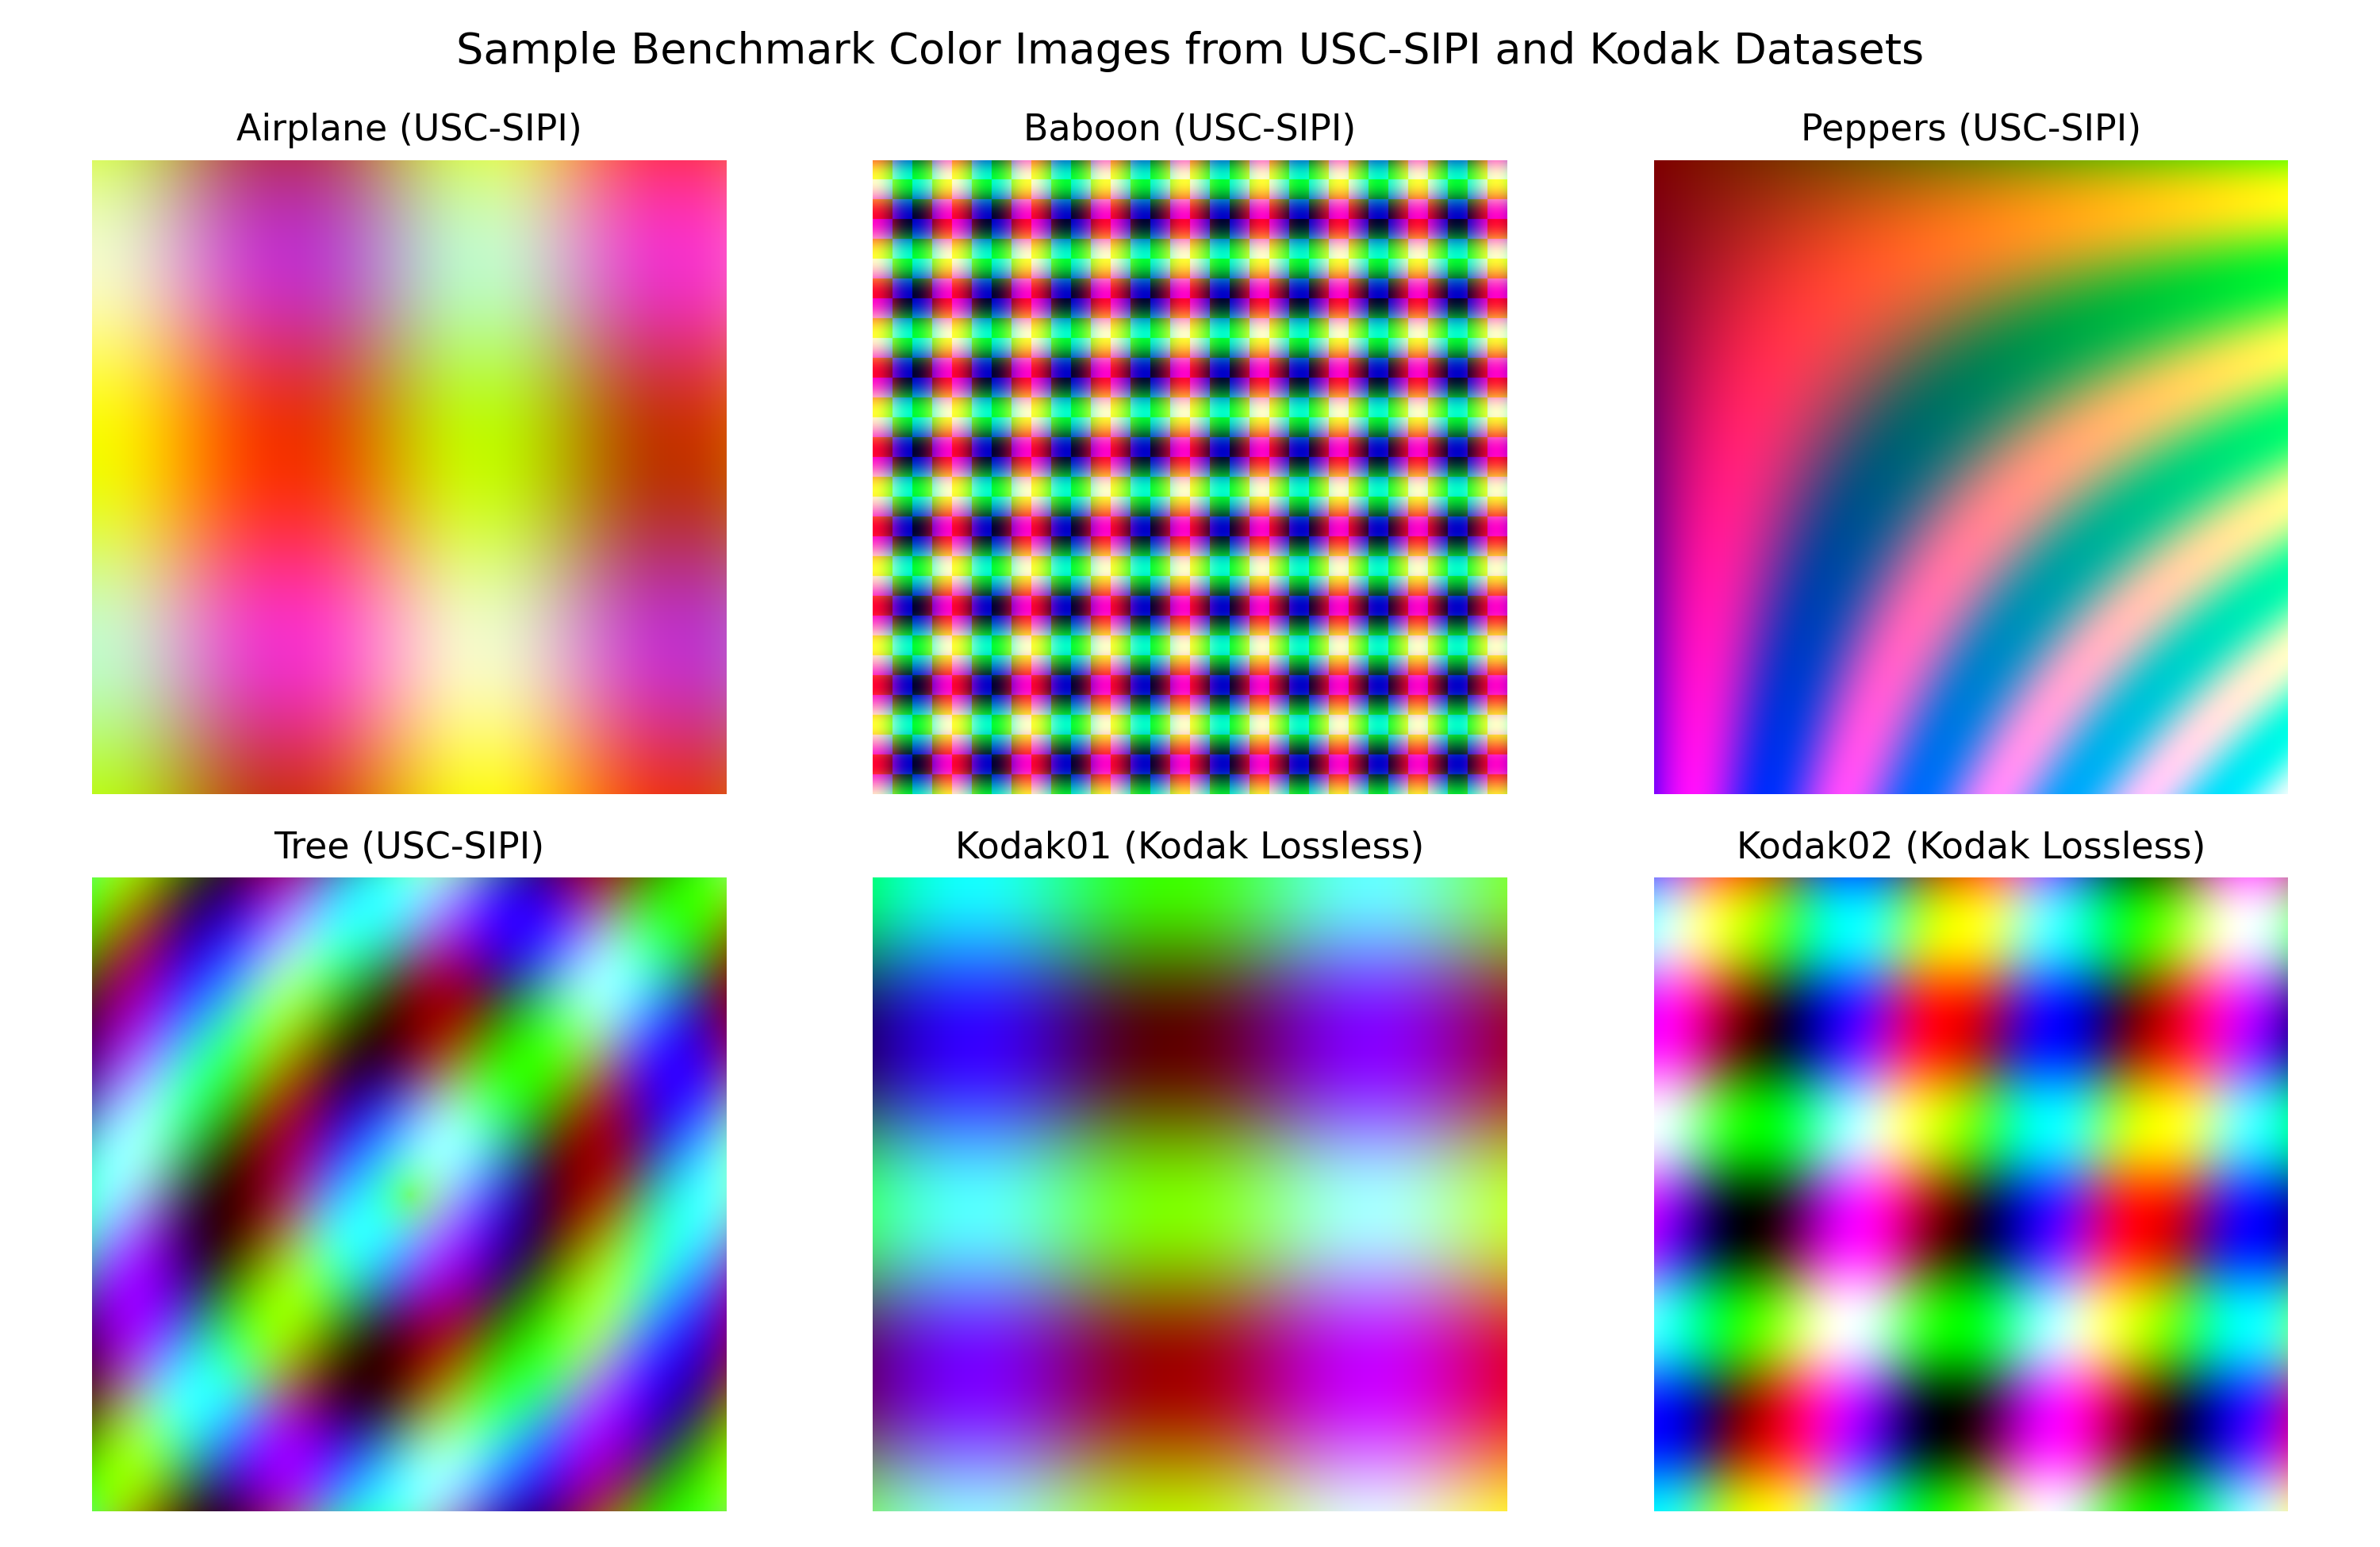
\includegraphics[width=0.88\textwidth]{images/dataset_samples.png}
    \caption[تصاویر آزمایشی استاندارد از پایگاه‌های داده \lr{USC-SIPI} و \lr{Kodak}]{نمونه تصاویر آزمایشی استاندارد منتخب از پایگاه‌های داده \lr{USC-SIPI} و \lr{Kodak} با تنوع بافتی و ساختار رنگی}
    \label{fig:dataset_samples}
\end{figure}

\section{معیارهای ارزیابی کمی عملکرد}

عملکرد الگوریتم بر اساس چهار دسته معیار کمی و آماری استاندارد ارزیابی می‌شود:

\subsection{آنتروپی شانون}

آنتروپی شانون ($H$) اصلی‌ترین معیار سنجش درجه تصادفی‌بودن و غیرقابل پیش‌بینی بودن توزیع مقادیر پیکسل‌ها در تصویر است. برای یک تصویر رنگی با عمق رنگی ۸ بیت در هر کانال، رابطه آنتروپی شانون به‌صورت زیر تعریف می‌شود:
\begin{equation}
H = -\sum_{i=0}^{255} p_i \log_2(p_i)
\label{eq:ch3-entropy}
\end{equation}
که در آن:
\begin{itemize}
    \item $i \in \{0, 1, \dots, 255\}$ نمایانگر ۲۵۶ سطح شدت روشنایی ممکن برای پیکسل‌ها در عمق ۸ بیتی است.
    \item $p_i$ احتمال وقوع و فراوانی نسبی سطح روشنایی $i$ام در کانال رنگی تصویر است ($\sum p_i = 1$).
    \item $\log_2$ لگاریتم در مبنای ۲ است که یکای آنتروپی را بر حسب بیت (\lr{bit}) مشخص می‌سازد.
    \item مقدار آرمانی نظری برای یک تصویر کاملاً تصادفی و یکنواخت برابر با $H = \log_2(256) = 8$ بیت است.
\end{itemize}

\subsection{ضریب همبستگی پیکسل‌های مجاور}

این ضریب میزان وابستگی و ارتباط خطی میان مقادیر جفت پیکسل‌های همسایه را در سه راستای افقی، عمودی و قطری اندازه می‌گیرد. رابطه محاسبه ضریب همبستگی پیرسون برابر است با:
\begin{equation}
r_{xy} = \frac{\sum_{i=1}^{M} (x_i - \bar{x})(y_i - \bar{y})}{\sqrt{\sum_{i=1}^{M} (x_i - \bar{x})^2 \sum_{i=1}^{M} (y_i - \bar{y})^2}}
\label{eq:ch3-corr}
\end{equation}
که در آن:
\begin{itemize}
    \item $x_i$ و $y_i$ مقادیر روشنایی دو پیکسل مجاور در جفت $i$ام هستند.
    \item $\bar{x} = \frac{1}{M}\sum_{i=1}^M x_i$ و $\bar{y} = \frac{1}{M}\sum_{i=1}^M y_i$ به ترتیب میانگین مقادیر $x_i$ و $y_i$ در نمونه $M$تایی از جفت‌های انتخابی هستند.
    \item در تصاویر اصلی طبیعی، $r_{xy} \approx 1$ است؛ در حالی که در تصویر رمزنگاری‌شده ایده‌آل باید $r_{xy} \approx 0$ باشد.
\end{itemize}

\subsection{معیارهای ارزیابی حساسیت تفاضلی (\lr{NPCR} و \lr{UACI})}

این دو معیار مقاومت الگوریتم را در برابر حملات تفاضلی ارزیابی می‌کنند و میزان تغییر خروجی در اثر تغییر تک‌بیتی در تصویر ورودی یا کلید را می‌سنجند:

\begin{enumerate}
    \item \textbf{نرخ تغییر تعداد پیکسل‌ها (\lr{NPCR}\footnote{\lr{Number of Pixels Change Rate}}):} درصد پیکسل‌هایی که مقادیر آن‌ها بین دو تصویر رمزشده تغییر کرده است:
    \begin{equation}
    \mathrm{NPCR} = \frac{\sum_{i=1}^H \sum_{j=1}^W D(i,j)}{W \times H} \times 100\%
    \label{eq:ch3-npcr}
    \end{equation}
    که در آن ماتریس دودویی $D(i,j)$ به‌صورت زیر تعریف می‌شود:
    \begin{equation}
    D(i,j) = \begin{cases}
    0, & C_1(i,j) = C_2(i,j) \\
    1, & C_1(i,j) \neq C_2(i,j)
    \end{cases}
    \end{equation}
    \item \textbf{میانگین شدت تغییر یکپارچه (\lr{UACI}\footnote{\lr{Unified Average Changing Intensity}}):} میانگین تفاوت مطلق مقادیر روشنایی پیکسل‌ها بین دو تصویر رمزشده:
    \begin{equation}
    \mathrm{UACI} = \frac{\sum_{i=1}^H \sum_{j=1}^W \left|C_1(i,j) - C_2(i,j)\right|}{255 \times W \times H} \times 100\%
    \label{eq:ch3-uaci}
    \end{equation}
\end{enumerate}
مقادیر آرمانی تئوریک عبارتند از $\mathrm{NPCR} > 99.60\%$ و $\mathrm{UACI} \approx 33.46\%$ که نشان‌دهنده حساسیت بهمنی عالی الگوریتم است\cite{ref10}.

\subsection{تحلیل پیچیدگی محاسباتی زمانی و فضایی}

فرض کنید ابعاد تصویر ورودی برابر با $H \times W$ و تعداد کل پیکسل‌ها $N = H \times W$ باشد:
\begin{itemize}
    \item \textbf{مرحله ۱ (آماده‌سازی):} پیچیدگی زمانی از مرتبه $O(N)$ است.
    \item \textbf{مرحله ۲ (جایگشت چن):} حل عددی $O(N)$ و مرتب‌سازی غیرمستقیم بردار پیوسته (\lr{argsort}) با الگوریتم مرتب‌سازی سریع نیازمند زمان $O(N \log N)$ است.
    \item \textbf{مرحله ۳ (انتخاب پویا):} تولید بردار انتخاب‌گر و یک گام سیستم نمایی در زمان خطی $O(N)$ انجام می‌گیرد.
    \item \textbf{مرحله ۴ و ۵ (انتشار دولایه \lr{XOR}):} هر دو لایه انتشار دارای پیچیدگی خطی $O(N)$ هستند.
\end{itemize}

بنابراین، پیچیدگی زمانی کل برای سه کانال رنگی برابر با $T(N) = O(N \log N)$ است و پیچیدگی فضایی به دلیل نگهداری ماتریس تصویر در حافظه برابر با $O(N)$ می‌باشد که کاملاً بهینه است.

\section{جمع‌بندی فصل}

در این فصل، معماری و جزئیات ریاضی الگوریتم رمزنگاری پیشنهادی تشریح شد. ویژگی‌های کلیدی طرح شامل استفاده از سیستم آشوبی چن برای جایگشت موقعیت مکانی، انتخاب پویای ۹ سیستم آشوبی نمایی برای لایه انتشار، انتشار دولایه مستقل \lr{XOR}، انطباق با اصل کرکوفس و فضای کلید ایمن $2^{350}$ است. در فصل چهارم، نتایج تجربی و تحلیل‌های آماری پیاده‌سازی این الگوریتم ارائه خواهد شد.